
%(BEGIN_QUESTION)
% Copyright 2003, Tony R. Kuphaldt, released under the Creative Commons Attribution License (v 1.0)
% This means you may do almost anything with this work of mine, so long as you give me proper credit

I henhold til ``Ohms lov'' for en kondensator er kondensatorstrøm proporsjonal med den {\it tidsderiverte} av kondensatorspenning:

$$i = C {dv \over dt}$$

En annen måte å si dette på er at kondensatorer {\it deriverer} spenning med hensyn på tid, og uttrykker denne {\it tidsderiverte} av spenning som en strøm. Dermed er strømmen ``gjennom'' en kondensator et uttrykk for hvor raskt spenningen {\it endrer seg} over tid.

\vskip 10pt

Anta at vi hadde et oscilloskop som kunne måle strøm direkte, eller i det minste en strøm-til-spenning-omformer vi kunne koble til en av probeinngangene slik at vi kunne måle strøm direkte på én kanal. Med et slikt instrumentoppsett kunne vi tegne kondensatorspenning og kondensatorstrøm direkte sammen på samme skjerm:

$$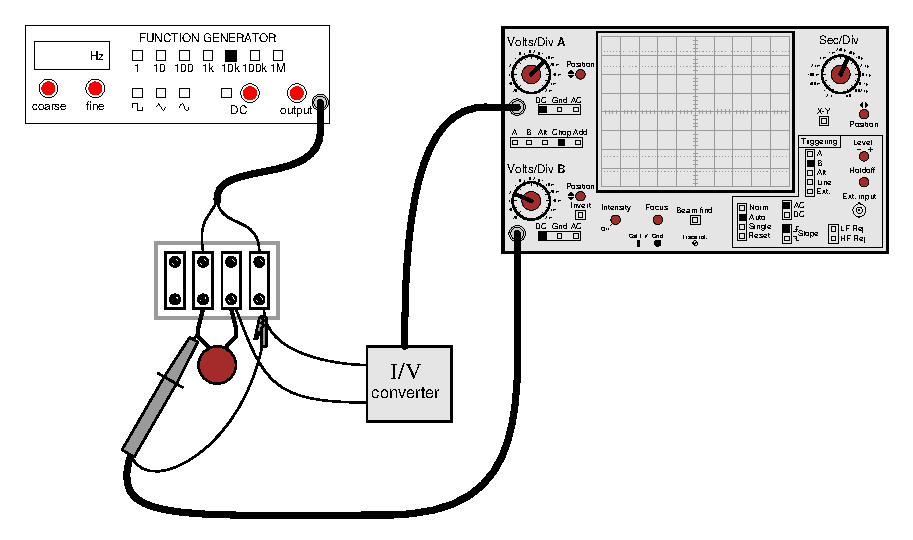
\includegraphics[width=15.5cm]{i01512x01.eps}$$

For hver av følgende spenningsbølgeformer (kanal B), tegn den tilsvarende kondensatorstrømbølgeformen (kanal A) slik den ville sett ut på oscilloskopskjermen:

$$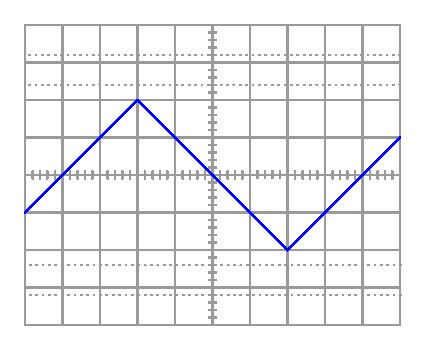
\includegraphics[width=15.5cm]{i01512x02.eps}$$

$$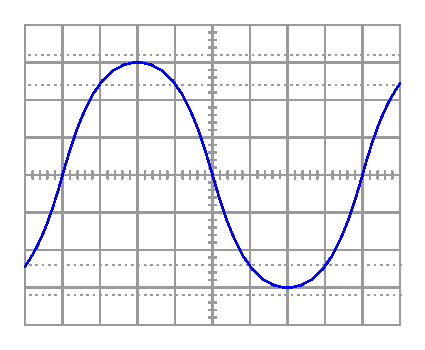
\includegraphics[width=15.5cm]{i01512x03.eps}$$

$$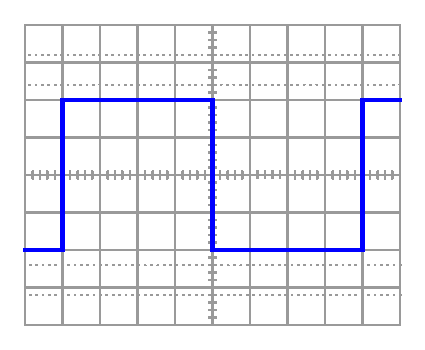
\includegraphics[width=15.5cm]{i01512x04.eps}$$

Merk: amplituden på strømplottene dine er valgfri, siden jeg ikke har gitt deg nok informasjon (kondensatorstørrelse osv.) til å faktisk {\it beregne} strømmen gjennom kondensatoren til ethvert tidspunkt. Det jeg er interessert i her er {\it formen} på hver strømbølgeform sammenlignet med {\it formen} på spenningsbølgeformen.

\underbar{file i01512}
%(END_QUESTION)





%(BEGIN_ANSWER)

$$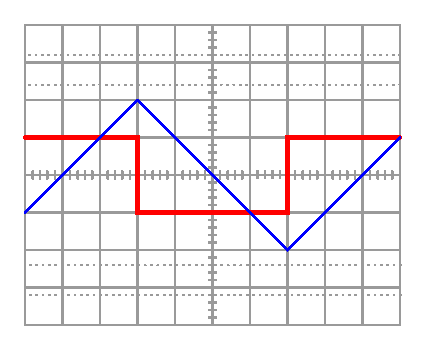
\includegraphics[width=15.5cm]{i01512x05.eps}$$

$$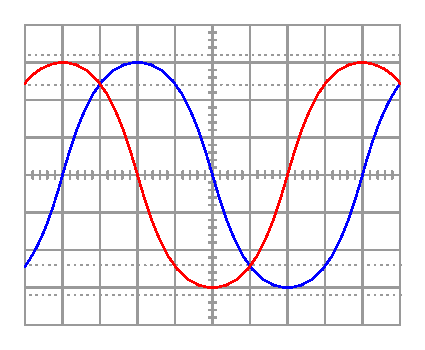
\includegraphics[width=15.5cm]{i01512x06.eps}$$

$$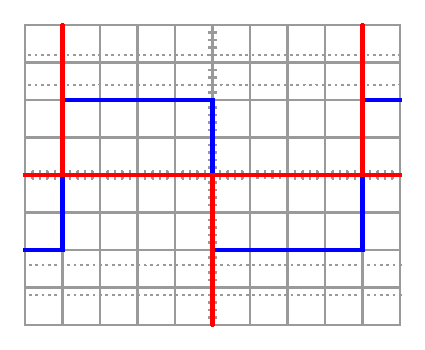
\includegraphics[width=15.5cm]{i01512x07.eps}$$

\vskip 10pt

Oppfølgingsspørsmål: Hvilken elektronisk komponent kan utføre funksjonen som en ``strøm-til-spenning-omformer'', slik at vi kan bruke et oscilloskop til å måle kondensatorstrøm? Vær så spesifikk som mulig i svaret.

%(END_ANSWER)





%(BEGIN_NOTES)

Her ber jeg studentene knytte den momentane endringsraten til spenningsbølgeformen til den momentane amplituden til strømbølgeformen. Bare en begrepsøvelse om deriverte.

%INDEX% Mathematics, calculus: derivative (defined in a graphical sense)

%(END_NOTES)

